\chapter{Prototipos de interfaz}
%En este capítulo adjunte y describa los prototipos de la interfaz para su aplicación. Procure hacer referencia al diseño de interacción y diseño para la usabilidad presentes en su aplicación.
%Si su aplicación tiene propiedades de accesibilidad para un público con necesidades especiales, por favor describa las estrategias usadas en esta sección.

En este capítulo se presentan los prototipos de interfaz desarrollados para la primera entrega del proyecto. El diseño busca mantener una apariencia sencilla y centrada en el documento, evitando mostrar permanentemente todas las herramientas disponibles. Las acciones principales se encuentran en el menú contextual y en el panel lateral, de manera que el área central pueda utilizarse principalmente para leer el PDF.

Los prototipos se dividen en dos áreas. La primera corresponde a la lectura y navegación de documentos PDF. La segunda reúne las funciones relacionadas con la gestión y edición básica de los archivos, como eliminar páginas, reordenarlas, guardarlas y combinar documentos.

\section{Prototipos de la funcionalidad de lectura y navegación de documentos PDF}
%Recuerde poner un texto introductorio breve para cada sección.
La pantalla principal de la aplicación está compuesta por el visor del documento y un conjunto reducido de controles. Al iniciar la aplicación sin ningún archivo abierto, se muestra una pantalla de bienvenida desde la cual el usuario puede seleccionar un PDF. Una vez abierto el documento, las páginas se renderizan de forma continua dentro del visor, permitiendo desplazarse verticalmente por todo el archivo.

En la parte superior se muestra el indicador de página actual junto con el número total de páginas. Este elemento también permite ingresar directamente el número de una página para desplazarse hasta ella. La aplicación cuenta además con controles de zoom, búsqueda de texto y selección de contenido, con el fin
de facilitar la lectura y la localización de información dentro de documentos extensos.

El panel lateral puede abrirse o cerrarse según sea necesario. Este panel contiene la lista de páginas y el outline del documento. La lista de páginas permite consultar las miniaturas y acceder rápidamente a una página específica.
Por otro lado, el outline muestra la estructura jerárquica del PDF cuando esta información se encuentra disponible. Al seleccionar una sección del outline, el visor se desplaza hasta la posición correspondiente.

La interfaz también incluye un menú contextual que se abre mediante el clic derecho. Este menú permite acceder a las funciones principales sin mantener una barra de herramientas visible durante la lectura. Entre sus opciones se encuentran abrir un archivo, guardar el documento, eliminar páginas, añadir
otro PDF y activar el modo de presentación.
\vspace{2cm}
\begin{figure}[H]
  \centering
    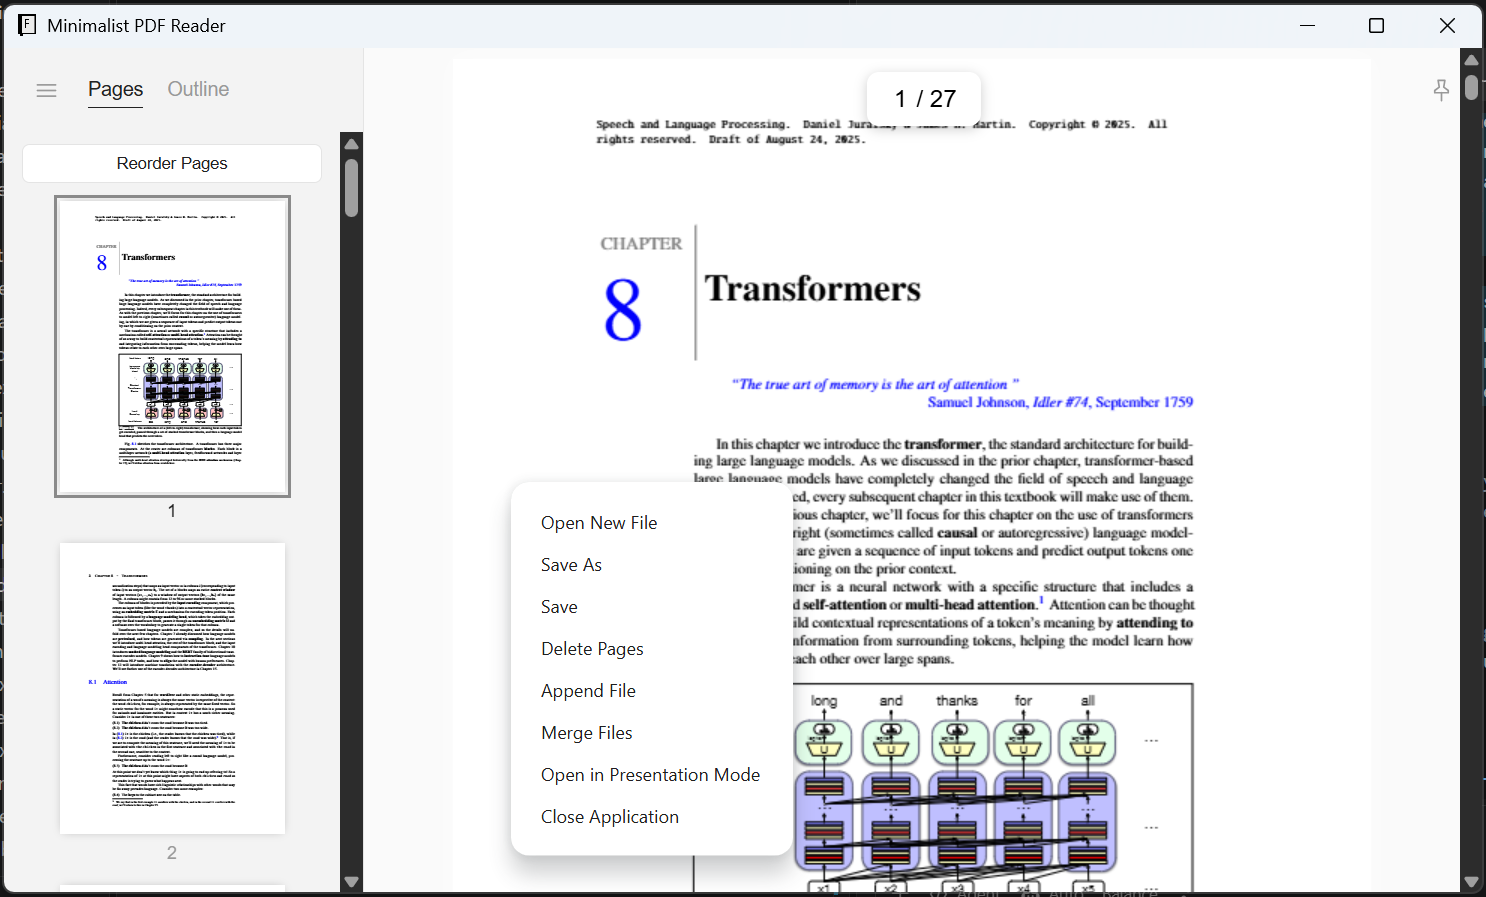
\includegraphics[height= 11cm, width=17cm]{project/images/prototipo1.png}
    \caption{Prototipo de la interfaz principal de lectura y navegación de documentos PDF.}
    \label{fig:prototipo de lectura y navegación 1}
\end{figure}
\newpage
\begin{figure}[H]
  \centering
    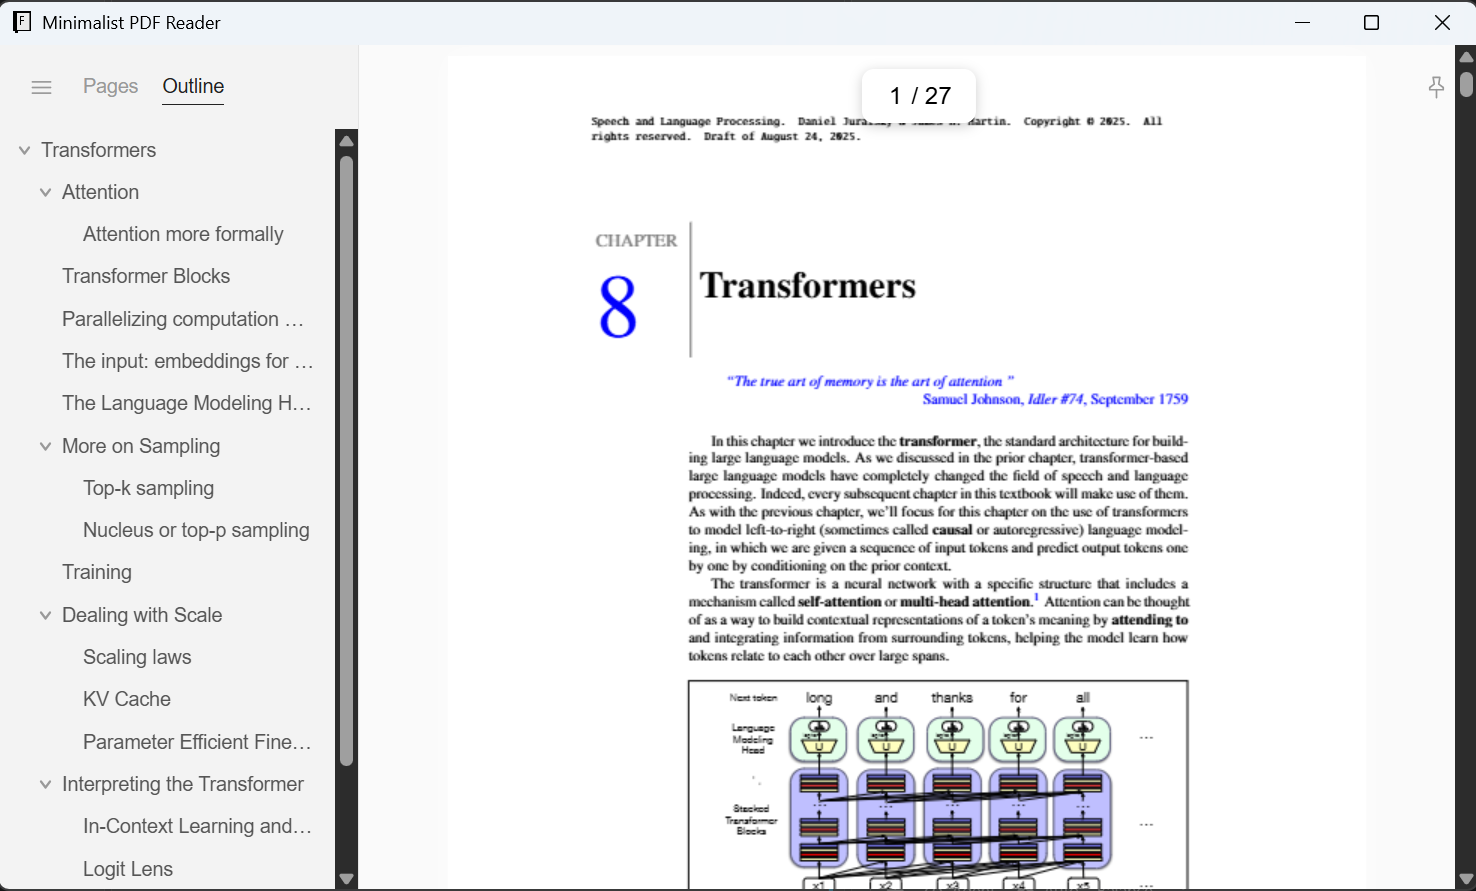
\includegraphics[height= 11cm, width=17cm]{project/images/prototipo2.png}
    \caption{Prototipo de la interfaz principal de lectura y navegación de documentos PDF.}
    \label{fig:prototipo de lectura y navegación 2}
\end{figure}
\vspace{1cm}

Como se muestra en la Figura \ref{fig:prototipo-lectura}, la interfaz mantiene el documento como elemento principal de la pantalla. Los controles se presentan solo cuando son necesarios, lo que permite conservar una apariencia ordenada y reducir las distracciones durante la lectura.

\section{Prototipos de la funcionalidad de gestión y edición básica de documentos}
%No olvide referenciar las imágenes en el texto usando \emph{label} y \emph{ref}.

La segunda área del prototipo corresponde a las funciones básicas de gestión y edición de documentos PDF. Estas funciones se acceden principalmente desde el menú contextual y desde el panel lateral de páginas, manteniendo la misma distribución general de la pantalla de lectura.

Para eliminar páginas, \ref{fig:prototipo-elim}, el usuario selecciona la opción correspondiente en el menú contextual. Luego se muestra un diálogo donde puede indicar las páginas que desea eliminar. Después de confirmar la operación, el documento se actualiza y el visor vuelve a cargar el contenido sin las páginas seleccionadas.

El panel lateral también permite activar el modo de reordenamiento \ref{fig:prototipo de lectura y navegación 1}. En este modo, el usuario puede arrastrar las miniaturas de las páginas para cambiar su posición dentro del documento. Una vez terminado el proceso, se guarda el nuevo orden y el PDF se actualiza con la estructura indicada.

La aplicación incluye dos opciones para guardar los cambios. La opción ``Save`` permite sobrescribir el archivo original, mientras que ``Save As``, \ref{fig:prototipo-saveas}, permite crear un nuevo documento y conservar el archivo original sin modificaciones. Esta última opción también se utiliza cuando el documento resulta de la combinación de varios archivos PDF.

El prototipo contempla además la posibilidad de añadir otro archivo PDF al documento actual, \ref{fig:prototipo-app}. El archivo seleccionado se concatena al final del documento abierto y el resultado puede guardarse como un nuevo PDF. Para la combinación de documentos se genera una vista previa, de modo que el usuario pueda revisar el resultado antes de guardarlo.

\begin{figure}[H]
  \centering
    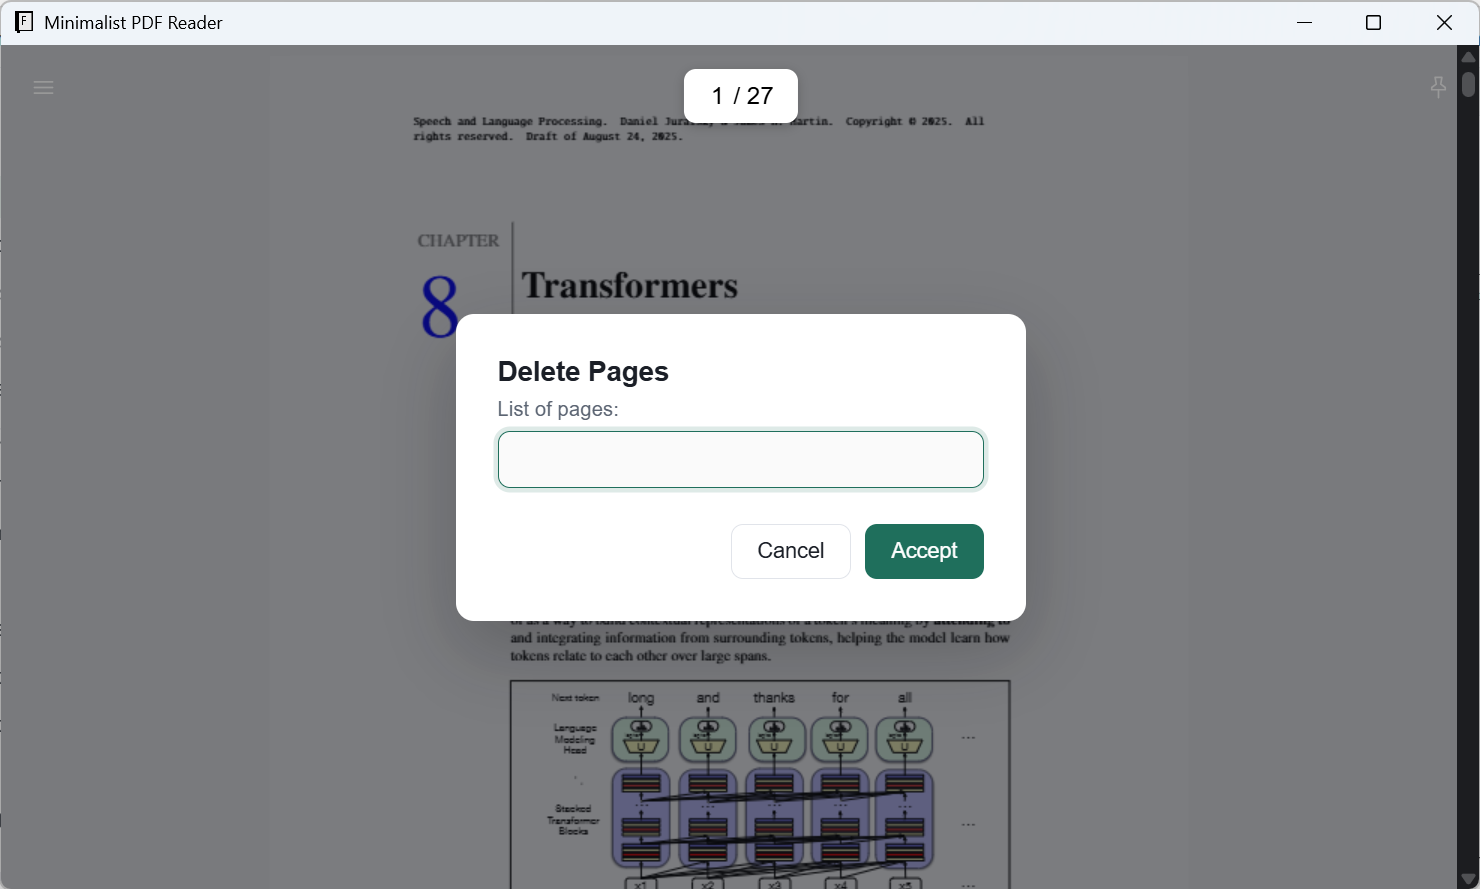
\includegraphics[height= 11cm, width=17cm]{project/images/protipo3Elim.png}
    \caption{Prototipo de eliminar página del PDF.}
    \label{fig:prototipo-elim}
\end{figure}

\begin{figure}[H]
  \centering
    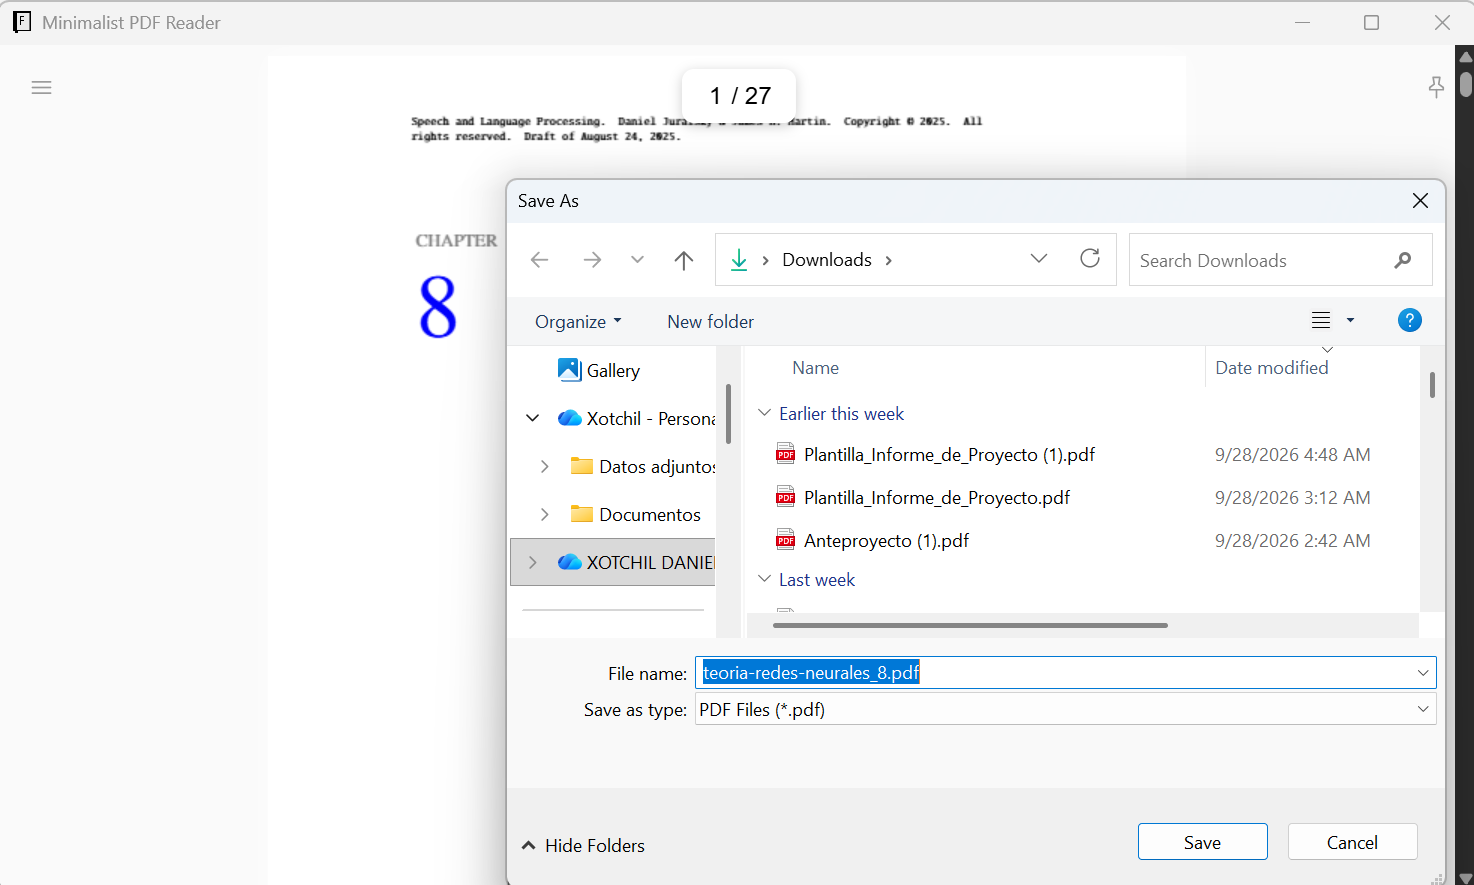
\includegraphics[height= 11cm, width=17cm]{project/images/prototipo4.SaveAs.png}
    \caption{Prototipo de guardar como.}
    \label{fig:prototipo-saveas}
\end{figure}

\begin{figure}[H]
  \centering
    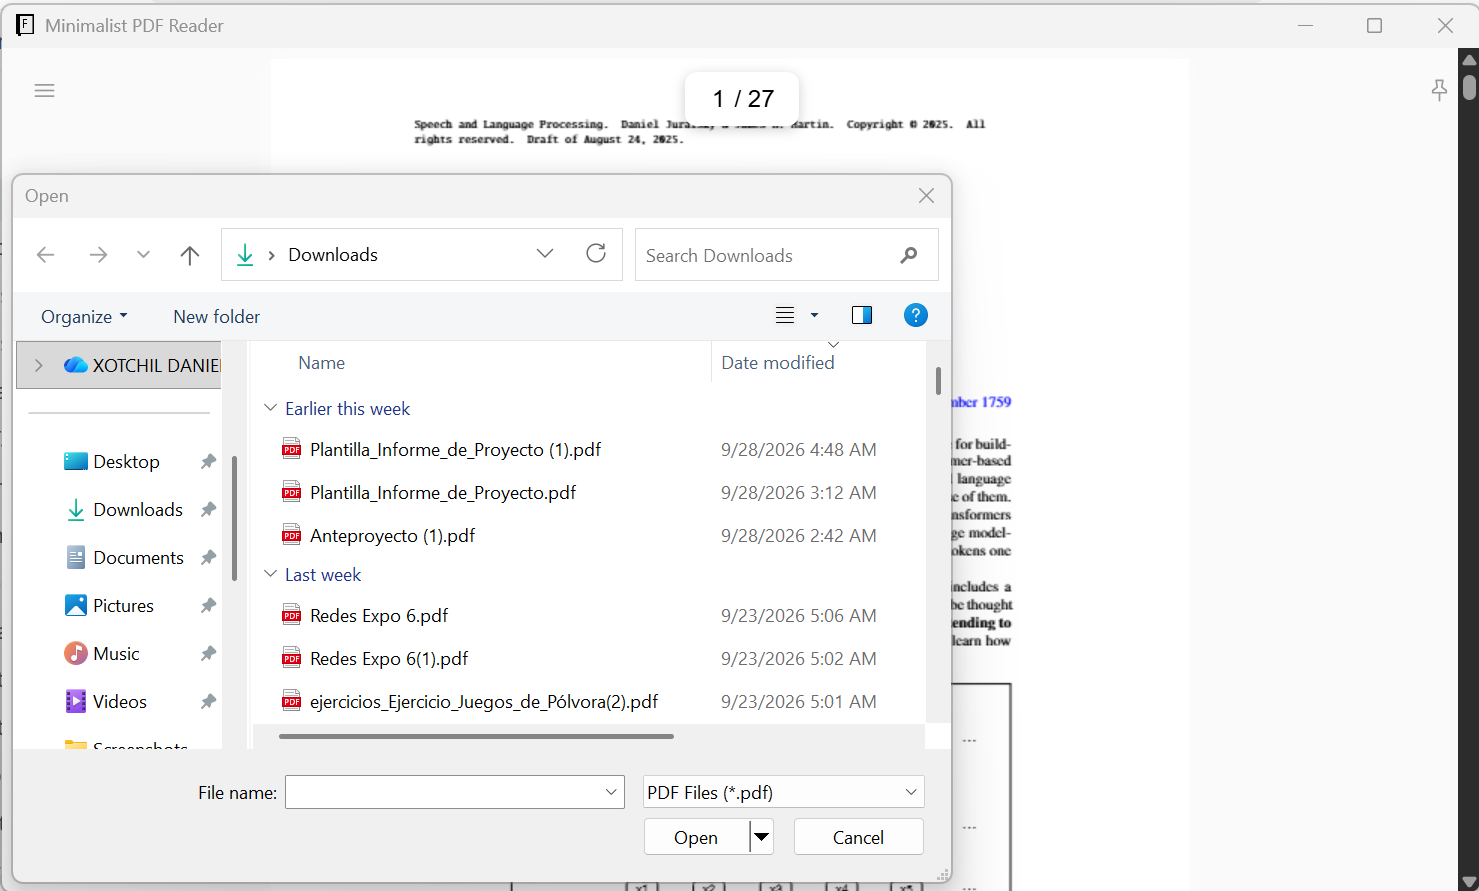
\includegraphics[height= 11cm, width=17cm]{project/images/prototipo5Append.png}
    \caption{Prototipo de agregar PDF.}
    \label{fig:prototipo-app}
\end{figure}

\begin{figure}[H]
  \centering
    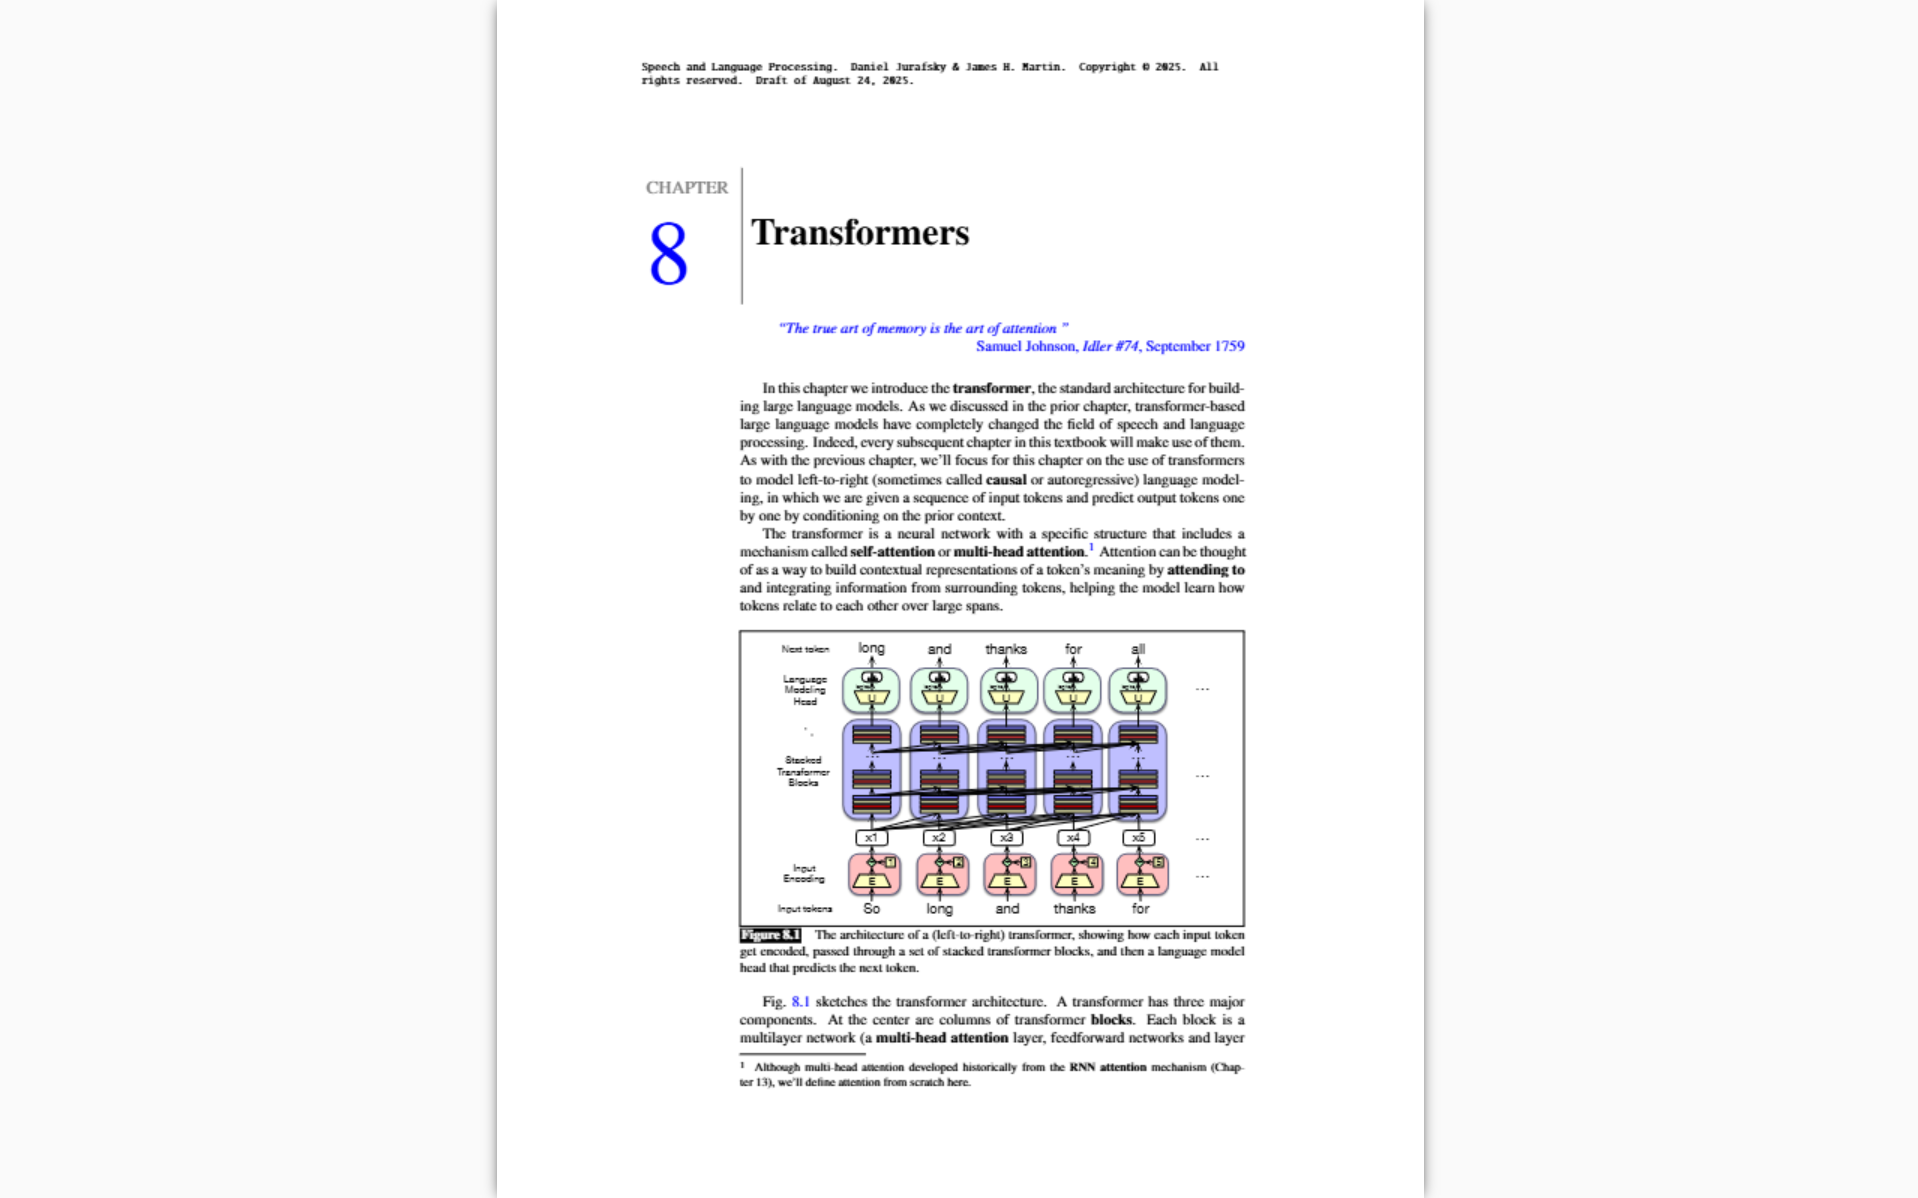
\includegraphics[height= 11cm, width=17cm]{project/images/prototipo6ModoPre.png}
    \caption{Prototipo de modo presentación del PDF.}
    \label{fig:prototipo-pres}
\end{figure}

\begin{figure}[H]
  \centering
    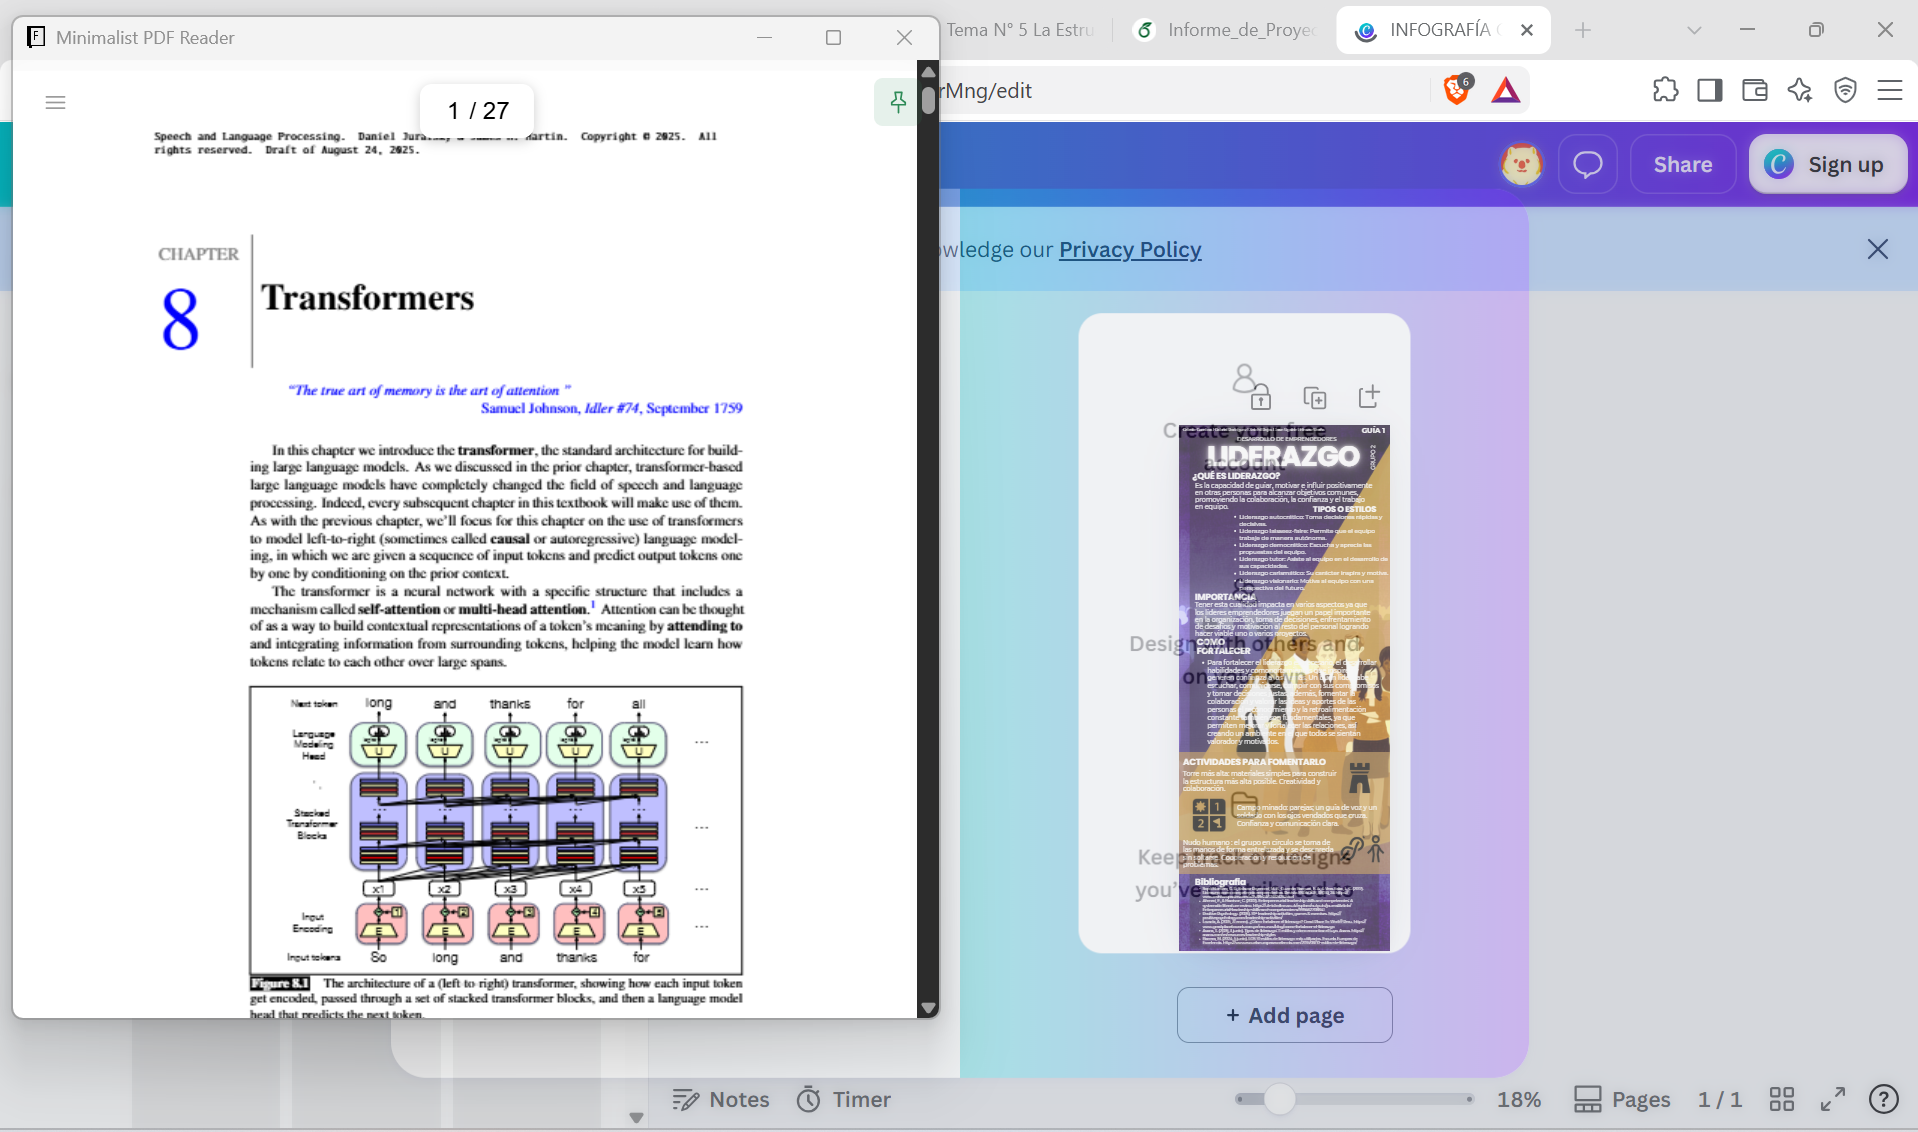
\includegraphics[height= 11cm, width=17cm]{project/images/prototipo6Flot.png}
    \caption{Prototipo de modo ajustado con comportamiento flotante PDF.}
    \label{fig:prototipo-aj}
\end{figure}
